\RequirePackage{luatex85,shellesc}

\documentclass[10pt]{beamer}
%\documentclass[aspectratio=169]{beamer}
\usetheme[background=light,numbering=fraction]{metropolis}           % Use metropolis theme
%\usetheme[background=light]{metropolis}           % Use metropolis theme
\usepackage{appendixnumberbeamer}

\usepackage{tikz}
\usetikzlibrary{fit, arrows.meta, calc, external}
%\tikzexternalize

\usepackage[super,negative]{nth}
\usepackage{url}
\usepackage{amssymb}
\usepackage{amsmath}
\usepackage{mathtools}
\usepackage[labelfont=bf,textfont={it}]{caption}
\usepackage{subcaption}
\captionsetup[figure]{justification=centering}
\captionsetup[subfigure]{justification=centering}
%\usepackage{subcaption}
%\usepackage[noindentafter]{titlesec}

\usepackage[maxnames=3,maxbibnames=99,mincrossrefs=5,style=trad-abbrv]{biblatex}
\addbibresource{../paper/mprop.bib}
% Make et al.s go all italic
\usepackage{xpatch}
\xpatchbibmacro{name:andothers}{%
	\bibstring{andothers}%
}{%
	\bibstring[\emph]{andothers}%
}{}{}
\DeclareFieldFormat{addendum}{}

\usepackage[binary-units]{siunitx}
\sisetup{range-phrase=--, range-units=single}
%\renewcommand{\deg}{\ensuremath{^{\circ}}\xspace}

\usepackage{microtype}
\usepackage{fontspec}
\usepackage{booktabs}
\usepackage{fontawesome}

\definecolor{graphc1}{RGB}{150,227,240}
\definecolor{graphc2}{RGB}{250,71,37}
\definecolor{graphc3}{RGB}{253,161,77}
\definecolor{graphc4}{RGB}{141,246,135}

% Official colours!

\definecolor{uofguniversityblue}{rgb}{0, 0.219608, 0.396078}

\definecolor{uofgheather}{rgb}{0.356863, 0.32549, 0.490196}
\definecolor{uofgaquamarine}{rgb}{0.603922, 0.72549, 0.678431}
\definecolor{uofgslate}{rgb}{0.309804, 0.34902, 0.380392}
\definecolor{uofgrose}{rgb}{0.823529, 0.470588, 0.709804}
\definecolor{uofgmocha}{rgb}{0.709804, 0.564706, 0.47451}

\definecolor{uofglawn}{rgb}{0.517647, 0.741176, 0}
\definecolor{uofgcobalt}{rgb}{0, 0.615686, 0.92549}
\definecolor{uofgturquoise}{rgb}{0, 0.709804, 0.819608}
\definecolor{uofgsunshine}{rgb}{1.0, 0.862745, 0.211765}
\definecolor{uofgpumpkin}{rgb}{1.0, 0.72549, 0.282353}
\definecolor{uofgthistle}{rgb}{0.584314, 0.070588, 0.447059}
\definecolor{uofgpillarbox}{rgb}{0.701961, 0.047059, 0}
\definecolor{uofglavendar}{rgb}{0.356863, 0.301961, 0.580392}

\definecolor{uofgsandstone}{rgb}{0.321569, 0.278431, 0.231373}
\definecolor{uofgforest}{rgb}{0, 0.317647, 0.2}
\definecolor{uofgburgundy}{rgb}{0.490196, 0.133333, 0.223529}
\definecolor{uofgrust}{rgb}{0.603922, 0.227451, 0.023529}

\newcommand{\lesspreceq}[1]{\prescript{}{#1}{\preceq}\ }

\title{Graph Models and Maximum Common Subgraph for Character Analysis}
\date{\nth{18} April, 2017}
\author{
	Kyle A. Simpson (2029567s) \\
	\tiny{\faGithub{} \url{https://github.com/FelixMcFelix} \hspace{0.5em} \faGlobe{} \url{https://mcfelix.me}}
}
\institute{University of Glasgow}

\begin{document}
\maketitle

%\begin{frame}{Table of contents}
%	\setbeamertemplate{section in toc}[sections numbered]
%	\tableofcontents[hideallsubsections]
%\end{frame}

\section{The Problem}

\begin{frame}{Modern Computer Vision Models}
%	\only<1|handout:1>{%
		For modern computer vision tasks, machine learning models and vector-space representations dominate.
		Typically these capture high-dimensional keypoints, consider low-level codings and/or learn data features through statistical inference.
		These are powerful approaches with proven effectiveness.
		
		\pause
		
		\begin{alertblock}{But...}
			\begin{itemize}[<+(1)- | alert@+(1)>]
				\item Popular representations are high-dimension vectors of real values---it can be hard to intuit their meaning!
				\begin{itemize}
					\item We can't look at e.g., a convolution kernel, and see what transformation it represents.
				\end{itemize}
				\item How can we then reason about a dependent system's robustness? Sensitive to odd phenomena; can be exploited by \emph{adversarial images} \cite{AdversarialML}.
			\end{itemize}
		\end{alertblock}
%	}%
\end{frame}

\begin{frame}{Why Graph Models?}
	\begin{columns}
		\begin{column}{0.6\linewidth}
			Graph models decompose problems into \alert{elements} and their \alert{relationships}---a sensible encoding for many domains.
			We can benefit greatly if they can be used sensibly within computer vision:
			
			\begin{itemize}[<+(1)- | alert@+(1)>]
				\item More intuitive problem models.
				\begin{itemize}
					\item We can manually assess whether a representation matches image content, and correct if need be.
				\end{itemize}
				\item Easier to assess model robustness.
				\item We can use standard, well-understood graph search and similarity algorithms, \emph{independent of domain}!
			\end{itemize}
		\end{column}
	
		\begin{column}{0.4\linewidth}
			\begin{figure}
			\centering
			\resizebox{\linewidth}{!}{
				\huge
				\begin{tikzpicture}
				\node[inner sep=5pt] (sagrada1) at (0,0)
				{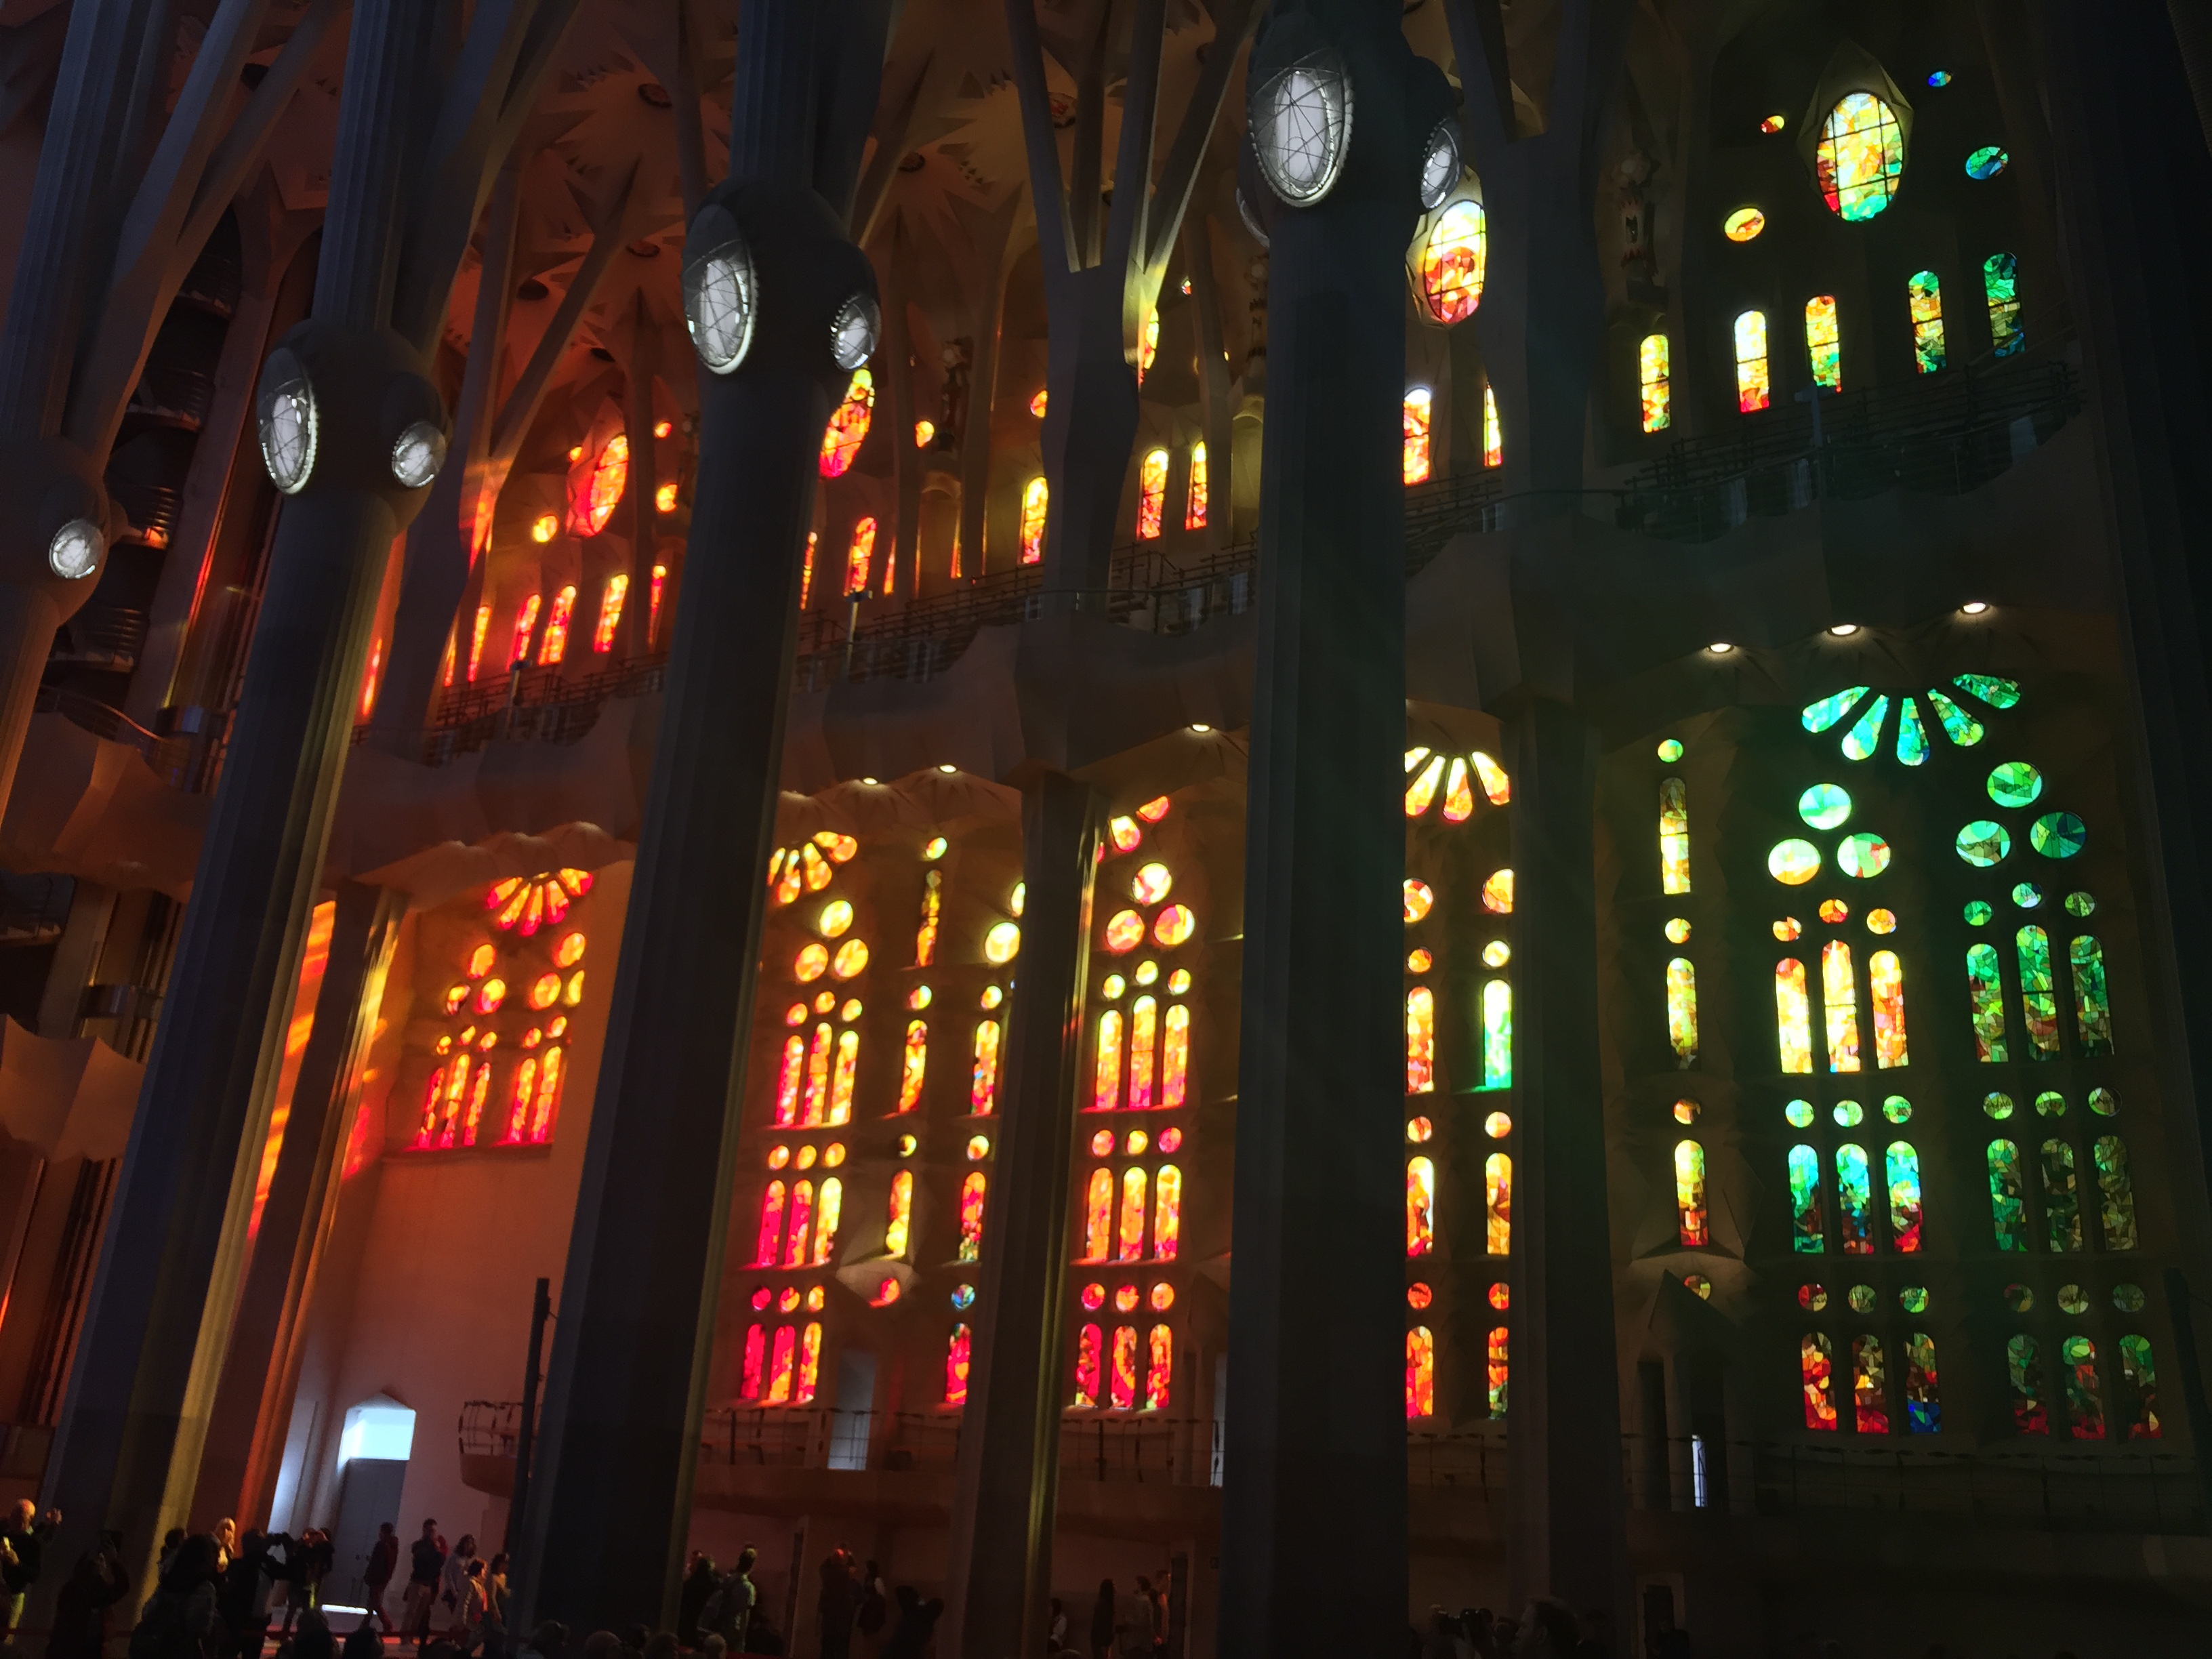
\includegraphics[width=0.9\linewidth]{../paper/images/IMG_3267.JPG}};
				\node[inner sep=5pt] (sagrada2) at (10,0)
				{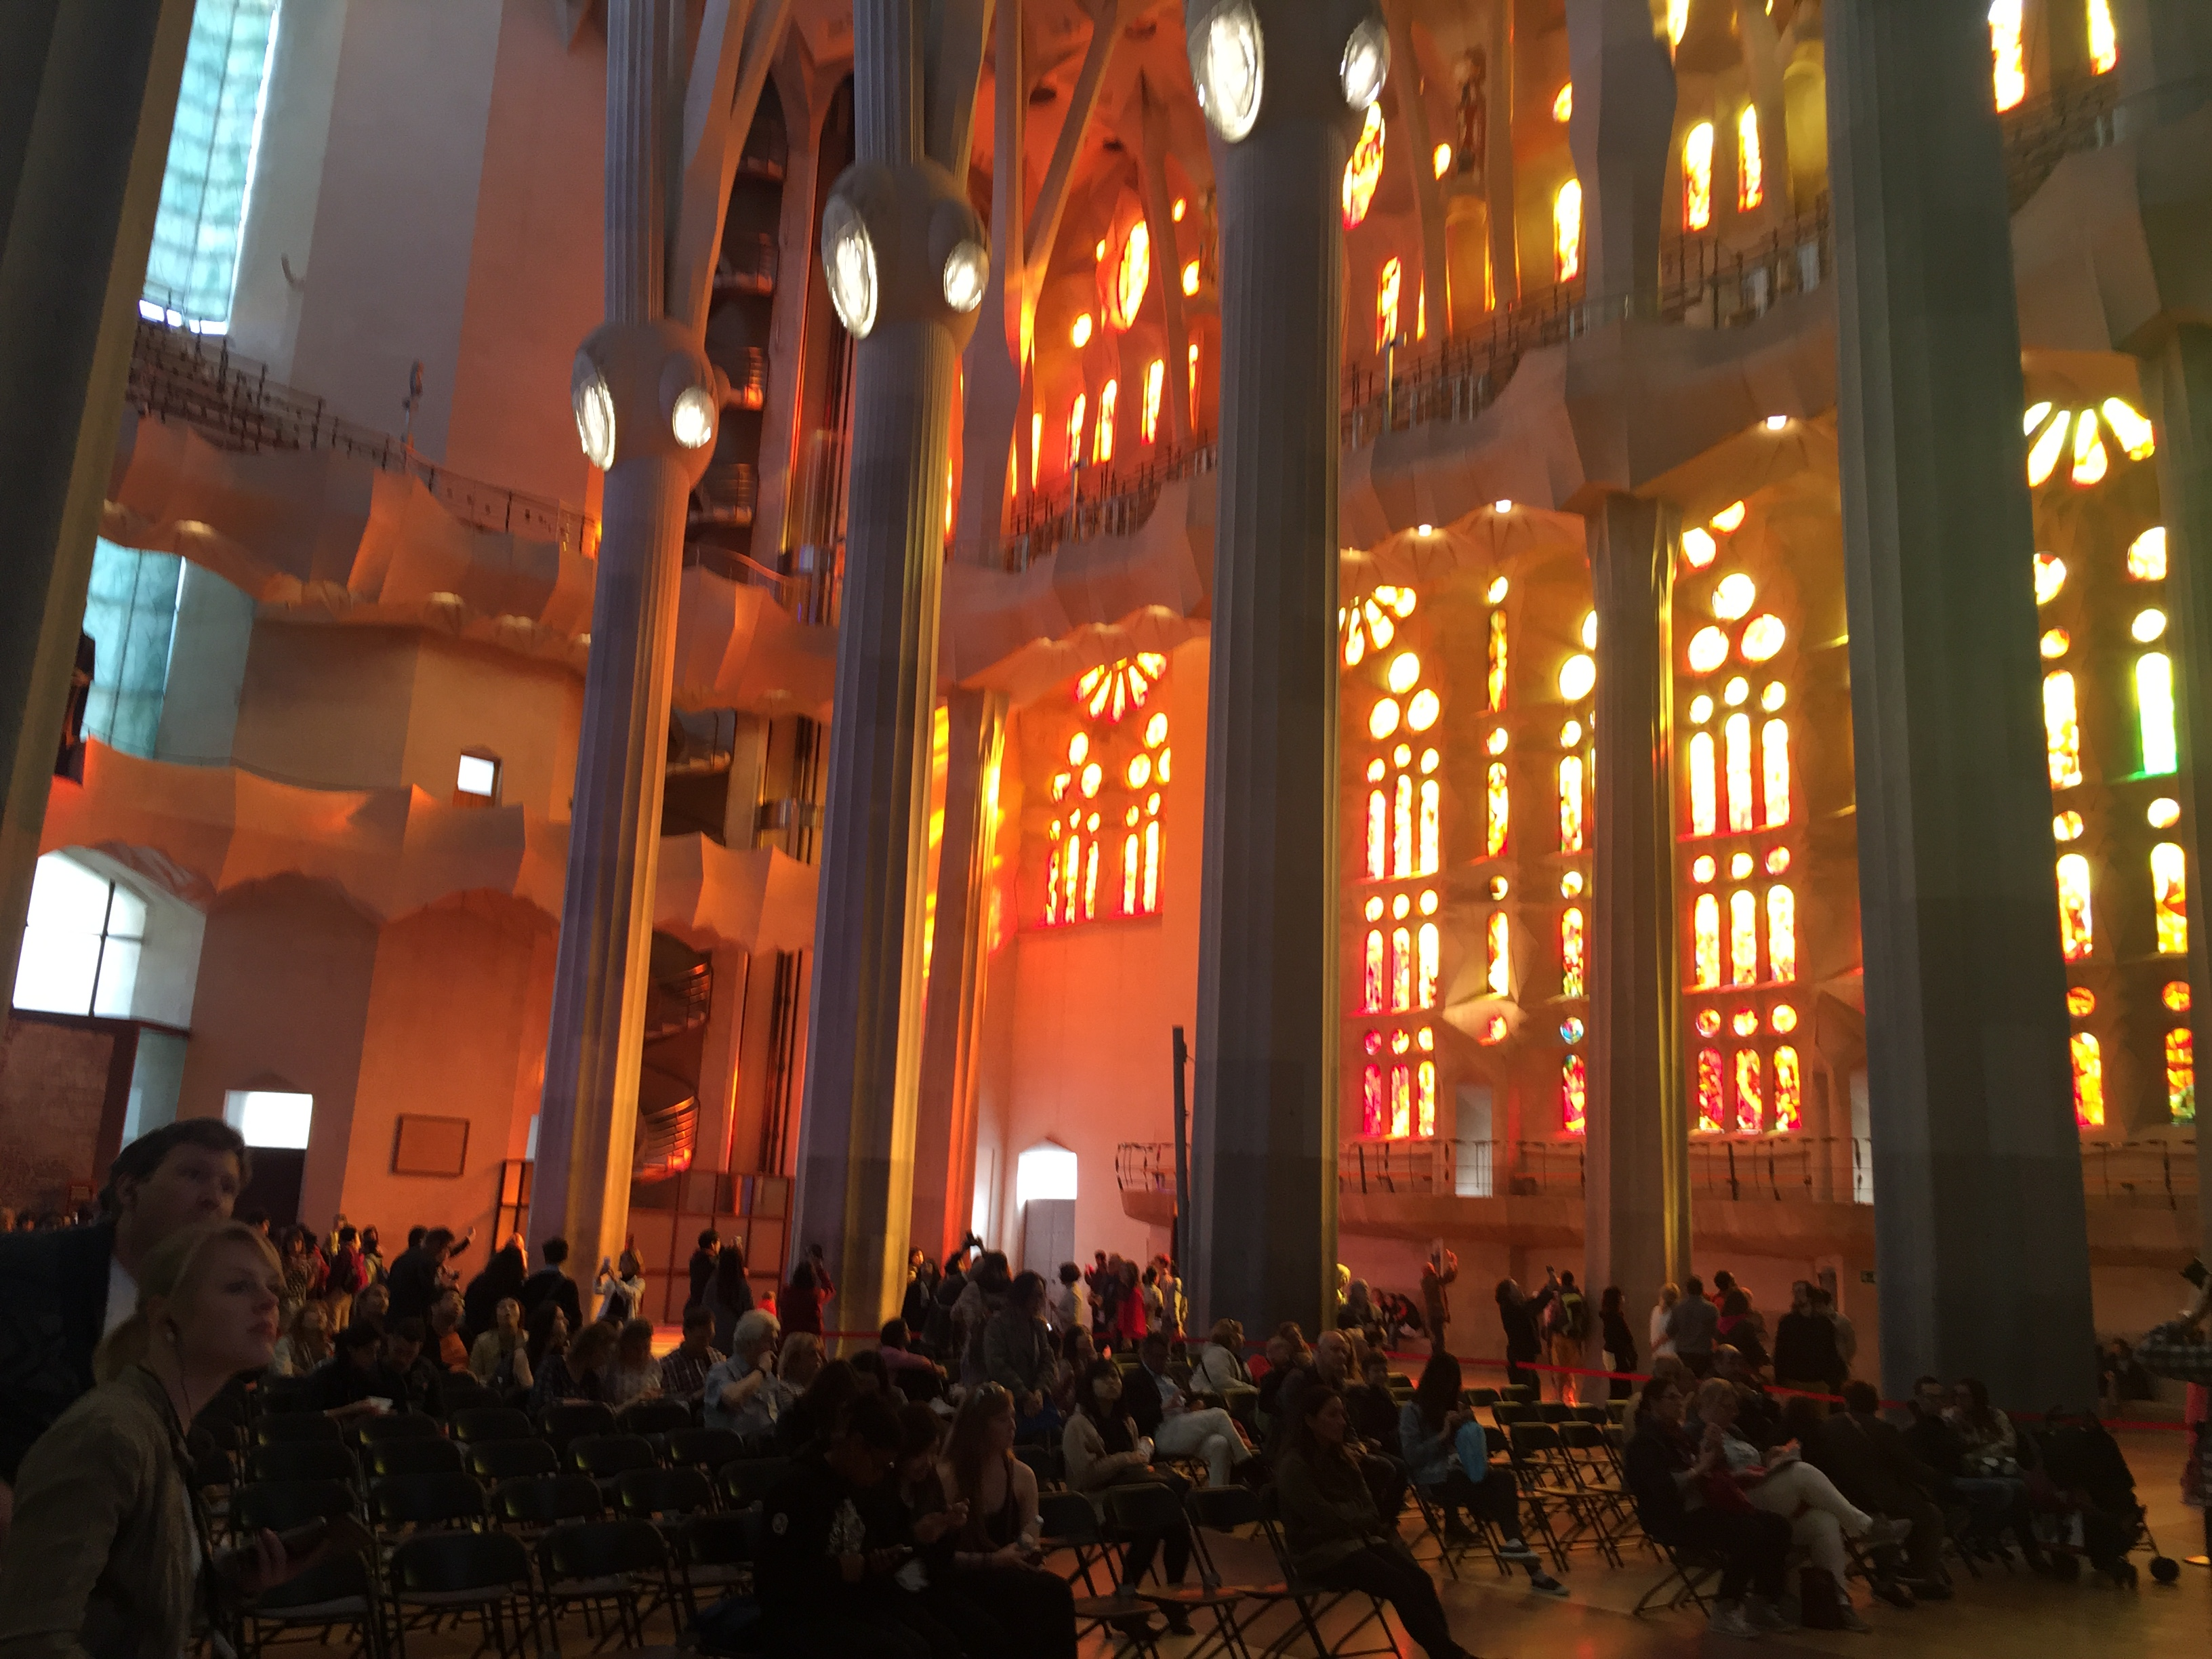
\includegraphics[width=0.9\linewidth]{../paper/images/IMG_3268.JPG}};
				
				\node[inner sep=5pt] (graph1) at (0,-6)
				{
					\begin{tikzpicture}
					\node[draw, circle, fill=graphc2] (n1) at (0,-1) {};
					\node[draw, circle, fill=graphc3] (n2) at (1,-0.67) {};
					\node[draw, circle, fill=graphc4] (n3) at (2,-0.33) {};
					\node[draw, circle, fill=graphc2] (n4) at (0,-2) {};
					\node[draw, circle, fill=graphc3] (n5) at (1,-1.9) {};
					\node[draw, circle, fill=graphc4] (n6) at (2,-1.8) {};
					
					\draw[<->] (n1) -- (n2);
					\draw[<->] (n2) -- (n3);
					\draw[<->] (n1) -- (n4);
					\draw[<->] (n2) -- (n5);
					\draw[<->] (n4) -- (n5);
					\draw[<->] (n5) -- (n6);
					\end{tikzpicture}
				};
				
				\node[inner sep=5pt] (graph2) at (10,-6)
				{
					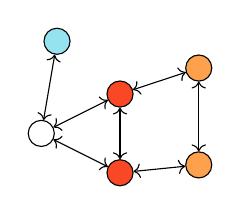
\begin{tikzpicture}
					\node[draw, circle] (n0) at (-1,-1.5) {};
					\node[draw, circle, fill=graphc1] (n7) at (-0.8,-0.33) {};
					\node[draw, circle, fill=graphc2] (n1) at (0,-1) {};
					\node[draw, circle, fill=graphc3] (n2) at (1,-0.67) {};
					\node[draw, circle, fill=graphc2] (n4) at (0,-2) {};
					\node[draw, circle, fill=graphc3] (n5) at (1,-1.9) {};
					
					\draw[<->] (n0) -- (n1);
					\draw[<->] (n0) -- (n4);
					\draw[<->] (n0) -- (n7);
					\draw[<->] (n1) -- (n2);
					\draw[<->] (n1) -- (n4);
					\draw[<->] (n2) -- (n5);
					\draw[<->] (n4) -- (n5);
					\end{tikzpicture}
				};
				
				\draw[->,thick] (sagrada1.east) -- (sagrada2.west)
				node[midway,fill=bg] {Similarity};
				\draw[->,thick] (graph1.east) -- (graph2.west)
				node[midway,fill=bg] {Similarity};
				
				\draw[->,thick] (sagrada1.south) -- (graph1.north)
				node[midway,fill=bg] {Transform};
				\draw[->,thick] (sagrada2.south) -- (graph2.north)
				node[midway,fill=bg] {Transform};
			\end{tikzpicture}}
			
			\caption{The core hypothesis---can we translate image similarity to graph similarity?}
			\end{figure}
		\end{column}
	\end{columns}
\end{frame}

\begin{frame}{Core Questions}
\begin{itemize}[<alert@+>]
	\item Are current graph models for generic image content suitable and/or effective?
	\item How useful is exact similarity (i.e.\ Maximum Common Subgraph) on new algorithms for simpler domain models?
	\begin{itemize}
		\item I.e. character recognition, word spotting.
	\end{itemize}
	\item How does this combination fare against existing graph models and similarity metrics in that domain?
\end{itemize}
\end{frame}

\section{Graph Similarity}

\begin{frame}{Quick Preliminaries}
	Given a graph $\mathcal{G}=(V,E)$, with vertex set $V$ and edge set $E$:
	
	\begin{itemize}[<+->]
		\item $\text{Ord}(\mathcal{G}) = |V|$, the vertex count or \emph{order} of $\mathcal{G}$
		\item $\text{Sz}(\mathcal{G}) = |E|$, the edge count or \emph{size} of $\mathcal{G}$
	\end{itemize}
\end{frame}

\begin{frame}{Subgraph Isomorphism: Graph Search}

\begin{columns}
\begin{column}{0.4\linewidth}
\begin{figure}
	\resizebox{\linewidth}{!}{\begin{tikzpicture}
	
	\node[label=below:{$\mathcal{P}$}] (p) at (0,0){
		\begin{tikzpicture}[scale=1]
		\begin{scope}[auto, every node/.style={draw,circle,minimum size=2em,inner sep=1},node distance=2cm]
		\node[draw, circle] (n1) at (0,0) {a};
		\node[draw, circle] (n2) at (0,-1) {c};
		\node[draw, circle] (n3) at (1,0) {b};
		\node[draw, circle] (n4) at (1,-1) {d};
		\end{scope}
		
		\draw[-] (n1) -- (n3);
		\draw[-] (n2) -- (n4);
		\draw[-] (n1) -- (n4);
		\draw[-] (n2) -- (n3);
		\draw[-] (n3) -- (n4);
		\end{tikzpicture}
	};
	
	\node[label=below:{$\mathcal{T}$}] (t) at (4,0){
		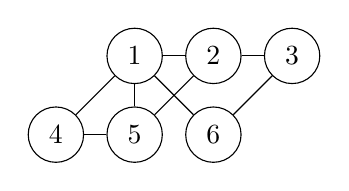
\begin{tikzpicture}[scale=1]
		\begin{scope}[auto, every node/.style={draw,circle,minimum size=2em,inner sep=1},node distance=2cm]
		\node[draw, circle] (n1) at (2,0) {2};
		\node[draw, circle] (n2) at (0,-1) {4};
		\node[draw, circle] (n3) at (1,0) {1};
		\node[draw, circle] (n4) at (1,-1) {5};
		
		\node[draw, circle] (n5) at (2,-1) {6};
		\node[draw, circle] (n6) at (3,0) {3};
		\end{scope}
		
		\draw[-] (n1) -- (n3);
		\draw[-] (n2) -- (n4);
		\draw[-] (n1) -- (n4);
		\draw[-] (n2) -- (n3);
		\draw[-] (n3) -- (n4);
		
		\draw[-] (n5) -- (n6);
		\draw[-] (n1) -- (n6);
		\draw[-] (n3) -- (n5);
		\end{tikzpicture}
	};
	
	\node[label=below:{Embedding}] (em) at (2,-3){
		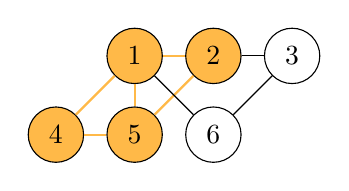
\begin{tikzpicture}[scale=1]
		\begin{scope}[auto, every node/.style={draw,circle,minimum size=2em,inner sep=1},node distance=2cm]
		\node[draw, circle, fill=uofgpumpkin] (n1) at (2,0) {2};
		\node[draw, circle, fill=uofgpumpkin] (n2) at (0,-1) {4};
		\node[draw, circle, fill=uofgpumpkin] (n3) at (1,0) {1};
		\node[draw, circle, fill=uofgpumpkin] (n4) at (1,-1) {5};
		
		\node[draw, circle] (n5) at (2,-1) {6};
		\node[draw, circle] (n6) at (3,0) {3};
		\end{scope}
		
		\draw[-, color=uofgpumpkin, thick] (n1) -- (n3);
		\draw[-, color=uofgpumpkin, thick] (n2) -- (n4);
		\draw[-, color=uofgpumpkin, thick] (n1) -- (n4);
		\draw[-, color=uofgpumpkin, thick] (n2) -- (n3);
		\draw[-, color=uofgpumpkin, thick] (n3) -- (n4);
		
		\draw[-] (n5) -- (n6);
		\draw[-] (n1) -- (n6);
		\draw[-] (n3) -- (n5);
		\end{tikzpicture}
	};
	
	\draw[->, thick] ($(em.north) + (0,1)$) -- (em.north);
	
	\end{tikzpicture}}

\caption{Example of SIP---$\mathcal{P}$'s embedding in $\mathcal{T}$ is shown in orange.}
\end{figure}
\end{column}

\begin{column}{0.6\linewidth}
	The \alert{subgraph isomorphism problem} (SIP): given a pattern graph $\mathcal{P}$ and a target graph $\mathcal{T}$, can we find a reproduction of $\mathcal{P}$ in $\mathcal{T}$?
	
	\begin{itemize}[<+(1)->]
		\item Non-induced? Preserves only adjacency. Can delete edges of $\mathcal{T}$ for embedding.
		\item Induced? Preserves both adjacency and non-adjacency---stricter matching!
		\item Feasible for graphs of order $10^3$.
	\end{itemize}
	
	\only<5->{
		I.e. can we find the image graph of a road sign inside a photograph?
	}
\end{column}

\end{columns}
\end{frame}

\begin{frame}{Maximum Common Subgraph: Graph Similarity}
\begin{columns}
	\begin{column}{0.65\linewidth}
		The \alert{maximum common subgraph problem} (MCS): given a pattern graph $\mathcal{P}$ and a target graph $\mathcal{T}$, what is the largest subgraph of $\mathcal{P}$ reproduced in $\mathcal{T}$?
		
		\begin{itemize}[<+(1)->]
			\item Induced and non-induced variants, as before.
			\item Feasible for graphs of order... 30--40.
			\item We now have a rough similarity metric: $\text{Ord}(\text{MCS}(\mathcal{P}, \mathcal{T}))$.
		\end{itemize}
		
		\only<5->{
			I.e. can we find the image graph of a road sign inside a photograph, where it is slightly obscured? (\emph{Occlusion invariant matching}).
		}
	\end{column}
	\begin{column}{0.35\linewidth}
		\begin{figure}
		\resizebox{\columnwidth}{!}{
			\begin{tikzpicture}
			
			\node[label=below:{$\mathcal{P}$}] (p) at (0,0){
				\begin{tikzpicture}[scale=1]
				\begin{scope}[auto, every node/.style={minimum size=2em,inner sep=1},node distance=2cm]
				\node[draw, circle] (n1) at (0,0) {a};
				\node[draw, circle] (n2) at (0,-1) {c};
				\node[draw, circle] (n3) at (1,0) {b};
				\node[draw, circle] (n4) at (1,-1) {d};
				
				\draw[-] (n1) -- (n3);
				\draw[-] (n2) -- (n4);
				\draw[-] (n1) -- (n4);
				\draw[-] (n2) -- (n3);
				\draw[-] (n3) -- (n4);
				\end{scope}
				\end{tikzpicture}
			};
			
			\node[label=below:{$\mathcal{T}$}] (t) at (3,0){
				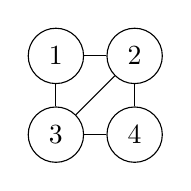
\begin{tikzpicture}[scale=1]
				\begin{scope}[auto, every node/.style={draw,circle,minimum size=2em,inner sep=1},node distance=2cm]
				\node[draw, circle] (n1) at (0,0) {1};
				\node[draw, circle] (n2) at (0,-1) {3};
				\node[draw, circle] (n3) at (1,0) {2};
				\node[draw, circle] (n4) at (1,-1) {4};
				\end{scope}
				
				\draw[-] (n1) -- (n3);
				\draw[-] (n2) -- (n4);
				\draw[-] (n1) -- (n2);
				\draw[-] (n2) -- (n3);
				\draw[-] (n3) -- (n4);
				
				\end{tikzpicture}
			};
			
			\node[label=below:{Embedding}] (em) at (1.5,-3){
				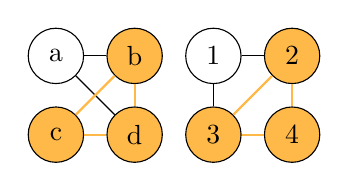
\begin{tikzpicture}[scale=1]
				\begin{scope}[auto, every node/.style={draw,circle,minimum size=2em,inner sep=1},node distance=2cm]
				\node[draw, circle] (n1) at (0,0) {a};
				\node[draw, circle, fill=uofgpumpkin] (n2) at (0,-1) {c};
				\node[draw, circle, fill=uofgpumpkin] (n3) at (1,0) {b};
				\node[draw, circle, fill=uofgpumpkin] (n4) at (1,-1) {d};
				
				\draw[-] (n1) -- (n3);
				\draw[-, color=uofgpumpkin, thick] (n2) -- (n4);
				\draw[-] (n1) -- (n4);
				\draw[-, color=uofgpumpkin, thick] (n2) -- (n3);
				\draw[-, color=uofgpumpkin, thick] (n3) -- (n4);
				
				\node[draw, circle] (n1') at (2,0) {1};
				\node[draw, circle, fill=uofgpumpkin] (n2') at (2,-1) {3};
				\node[draw, circle, fill=uofgpumpkin] (n3') at (3,0) {2};
				\node[draw, circle, fill=uofgpumpkin] (n4') at (3,-1) {4};
				
				
				\draw[-] (n1') -- (n3');
				\draw[-, color=uofgpumpkin, thick] (n2') -- (n4');
				\draw[-] (n1') -- (n2');
				\draw[-, color=uofgpumpkin, thick] (n2') -- (n3');
				\draw[-, color=uofgpumpkin, thick] (n3') -- (n4');
				\end{scope}
				\end{tikzpicture}
			};
			
			\draw[->, thick] ($(em.north) + (0,1)$) -- (em.north);
			
		\end{tikzpicture}}
		
		\caption{Example of MCS. The result's embedding in both $\mathcal{P}$ and $\mathcal{T}$ is shown in orange.}
		\end{figure}
	\end{column}
\end{columns}
\end{frame}

\begin{frame}{Graph Edit Distance: Graph Dissimilarity}
	We can count the number of vertex additions and deletions needed to transform $\mathcal{P}$ into $\mathcal{T}$---the \alert{graph edit distance} (GED).
	
	$$ \text{GED}(\mathcal{P}, \mathcal{T}) = \text{Ord}(\mathcal{P}) + \text{Ord}(\mathcal{T}) - 2 \times \text{Ord}(\text{MCS}(\mathcal{P}, \mathcal{T})) $$
	
	This is the core metric used in this work---note that this gives edge changes zero cost.
\end{frame}

\section{State-of-the-art Generic Models}

\begin{frame}{State-of-the-art Generic Models}
\begin{itemize}%[<+->]
	\item Present work (such as \citeauthor{Plane-Graphs-From-Images} \cite{Plane-Graphs-From-Images} or \citeauthor{Submap-Iso-Images} \cite{Submap-Iso-Images}) focuses on building plane graphs for their algorithmic properties.
	\begin{itemize}
		\item They extract interest pixel locations then compute the \alert{Delaunay triangulation} \cite{Delaunay}, building a triangle mesh s.t.\ no point falls inside any triangle's circumcircle.
	\end{itemize}
	
	\item \citeauthor{Plane-Graphs-From-Images} attempt to extend this with structural cues from image segmentation.
	
	\item These don't appear to capture any discriminative features: these works focus on matching elements \emph{within} an image, and \textbf{not between images}. Is this the case?
\end{itemize}
\end{frame}

\begin{frame}{Putting \citeauthor{Plane-Graphs-From-Images} to the Test}
\begin{columns}
	\begin{column}{0.8\linewidth}
		I reimplemented their work, with two experiments in mind using the \alert{$k\downarrow$} MCS algorithm \cite{Between-MCS-SIP}:
		
		\begin{enumerate}[<alert@+(1)>]
			\item Is the graph of a test image from the Berkeley Segmentation Dataset rotated $180^{\circ}$ isomorphic to itself? I.e. is this transformation isotropic?
			
			\item How similar are two adjacent frames from Sergio Leone's \emph{The Good, the Bad and the Ugly}?
		\end{enumerate}
	
%		\only<4->{
		For this, I augment graphs with positional data, applying euclidean distance filtering to help matching along.
	%	In the first case, perfect segmentation information is known.
	%	In the second, this must be done algorithmically.
	\end{column}

	\begin{column}{0.2\linewidth}
		\begin{figure}
			\centering
			\begin{figure}
%				\only<2->{
				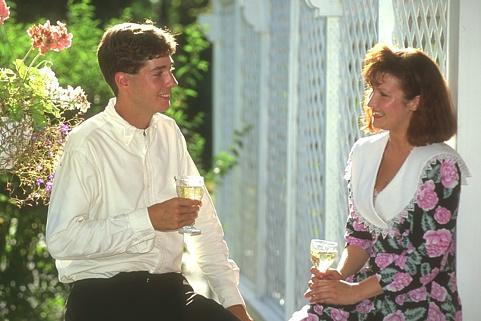
\includegraphics[width=\linewidth]{../paper/images/bsd-157055}
%				}
				
%				\only<3->{
				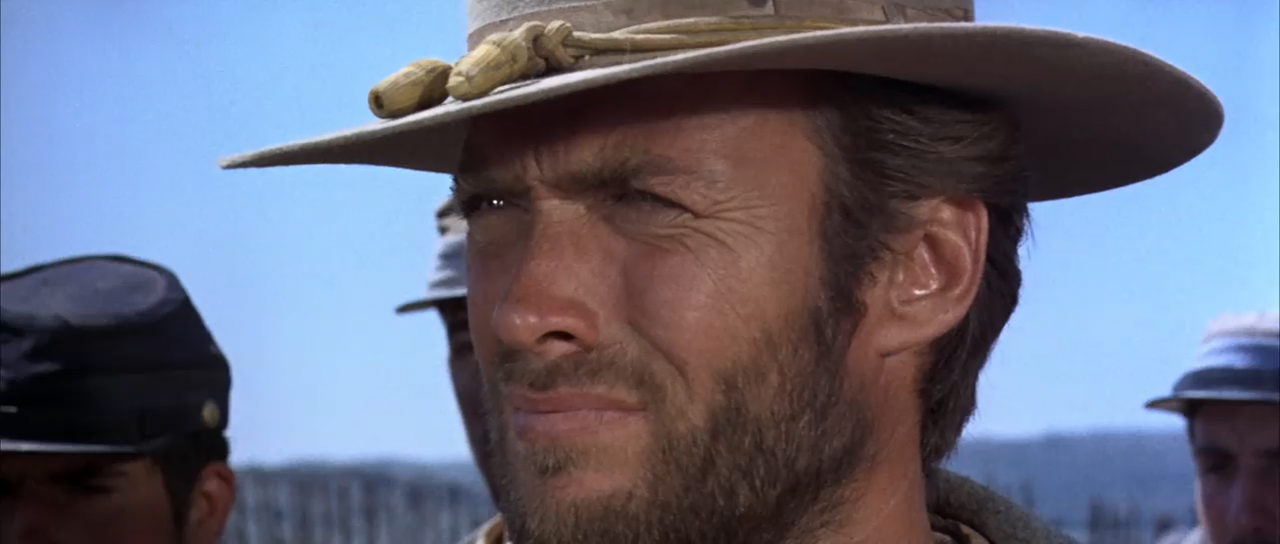
\includegraphics[width=\linewidth]{../paper/images/gbu2}
				
				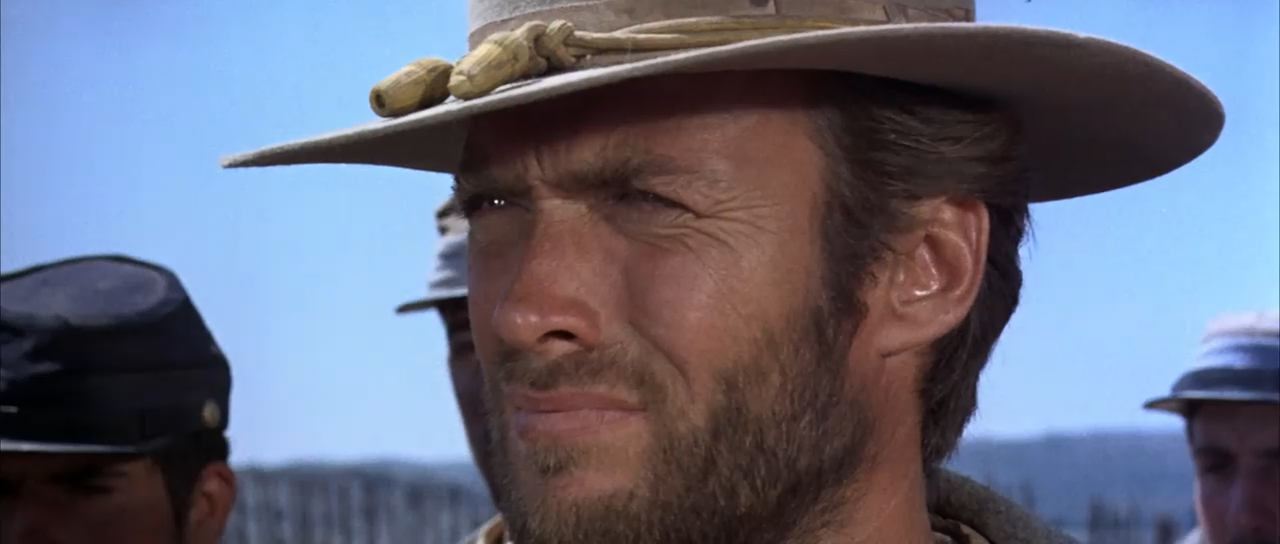
\includegraphics[width=\textwidth]{../paper/images/gbu3}
%				}
				
			\caption{Three test images: BSD, GBU1 and GBU2.}
			\end{figure}
		\end{figure}
	\end{column}
\end{columns}
\end{frame}

\begin{frame}{The Results?}
\begin{columns}
	\begin{column}{0.4\linewidth}
		\begin{table}[h]
			\centering
			\resizebox{0.7\linewidth}{!}{
				\begin{tabular}{lSS}
					\toprule
					\multicolumn{1}{c}{Image} & \multicolumn{1}{c}{Order} & \multicolumn{1}{c}{Size} \\ \midrule
					BSD & \num{245} & \num{707} \\
					BSD-180 & \num{247} & \num{705} \\
					GBU1 & \num{264} & \num{755} \\
					GBU2 & \num{260} & \num{743} \\
					\bottomrule
				\end{tabular}
			}
			
			\caption{
				Graph stats for real-world images.
			}
		\end{table}
		\begin{table}[h]
			\centering
			\resizebox{\linewidth}{!}{
			\begin{tabular}{cccc}
				\toprule
				Experiment & Except-$k$ & $\text{Ord}(\mathit{MCS})$ & Overlap (\si{\percent}) \\ \midrule
				1 & $[61, 111]$ & $[134, 184]$ & 54.6--72.2 \\
				2 & $[38, 217]$ & $[47, 226]$ & 18.1--86.9 \\
				\bottomrule
			\end{tabular}
			}
			
			\caption{
				Observed similarity bounds between real-world images.
				\label{tab:badgraphs}
			}
		\end{table}
	\end{column}

	\begin{column}{0.6\linewidth}
		Findings (after 5 days running on fatanode-01):
		\begin{itemize}[<+(1)-|alert@+(1)>]
			\item Negative results on both counts!
			\begin{itemize}
				\item \alert{No isomorphism in first experiment}, with lower similarity than expected.
				\item Wide bound in second experiment---\alert{uniform graph structure hinders matching performance}.
			\end{itemize}
			\item Not isotropic---inherits sensitivities from interest pixel detector.
			\item Depends heavily on perfect segmentation, to detriment of matching.
		\end{itemize}
	\end{column}
\end{columns}
\end{frame}

\frame[standout]{
	These are high-order, high-size graphs with uniform structure and no discriminative features.
	\alert{This approach is \emph{not} appropriate for real-world matching!}
}

\section{Let's Narrow our Scope: Character Glyph Modelling}

\begin{frame}{Matching Features}
	The main features I want to capture from characters (fonts or handwritten) are \alert{curves}, \alert{lines}, \alert{component topology} and \alert{orientation} to have a reasonably robust model.
\end{frame}

\begin{frame}{A Simple Algorithm: GlyphGraph}
\begin{columns}
	\begin{column}{0.4\linewidth}
		\only<4>{\vspace{-1.5em}}
		\begin{enumerate}[<alert@+>]
			\item Input Image
			\item Preprocessing (Thresholding, Skeletonisation)
			\item Connected Component Labelling
			\item Interest Point Location
			\item Path Traversal and Splitting (IPAN Algorithm \cite{PathCurvature})
			\item Topology and ``North'' Labelling
		\end{enumerate}
	\end{column}
	\begin{column}{0.6\linewidth}
		\def\pixels{
			{0,0,0,0,0,0,0,0,0,0,0},
			{0,0,0,0,1,1,1,0,0,0,0},
			{0,0,0,1,0,0,0,1,0,0,0},
			{0,0,1,0,0,0,0,0,1,0,0},
			{0,0,1,0,0,0,0,0,1,0,0},
			{0,0,1,0,1,1,1,0,1,0,0},
			{0,0,1,0,0,0,0,0,1,0,0},
			{0,0,1,0,0,0,0,0,1,0,0},
			{0,0,0,1,0,0,0,1,0,0,0},
			{0,0,0,0,1,1,1,0,0,0,0},
			{0,0,0,0,0,0,0,0,0,0,0}%
		}
		\def\comps{
			{0,0,0,0,0,0,0,0,0,0,0},
			{0,0,0,0,2,2,2,0,0,0,0},
			{0,0,0,2,0,0,0,2,0,0,0},
			{0,0,2,0,0,0,0,0,2,0,0},
			{0,0,2,0,0,0,0,0,2,0,0},
			{0,0,2,0,3,3,3,0,2,0,0},
			{0,0,2,0,0,0,0,0,2,0,0},
			{0,0,2,0,0,0,0,0,2,0,0},
			{0,0,0,2,0,0,0,2,0,0,0},
			{0,0,0,0,2,2,2,0,0,0,0},
			{0,0,0,0,0,0,0,0,0,0,0}%
		}
			
		\only<1|handout:1>{
			\begin{figure}
				\definecolor{pixel 0}{HTML}{FFFFFF}
				\definecolor{pixel 1}{HTML}{000000}
				\definecolor{pixel 4}{RGB}{150,227,240}
				\colorlet{pixel 3}{uofglavendar}
				\colorlet{pixel 2}{uofgpumpkin}
				\centering
				\resizebox{\linewidth}{!}{
					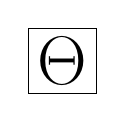
\begin{tikzpicture}
					\node[font=\fontsize{120}{120}\selectfont, draw] at (0,0) (Letter) {$\Theta$};
					\end{tikzpicture}
				}
				\caption{Glyph Image\label{fig:walkthrough:glyph}}
			\end{figure}
		}
	
		\only<2|handout:2>{
			\addtocounter{figure}{1}
			\begin{figure}
				\definecolor{pixel 0}{HTML}{FFFFFF}
				\definecolor{pixel 1}{HTML}{000000}
				\definecolor{pixel 4}{RGB}{150,227,240}
				\colorlet{pixel 3}{uofglavendar}
				\colorlet{pixel 2}{uofgpumpkin}
				\centering
				\resizebox{0.9\linewidth}{!}{
					\begin{tikzpicture}
					\foreach \line [count=\y] in \pixels {
						\foreach \pix [count=\x] in \line {
							\draw[fill=pixel \pix] (\x,-\y) rectangle +(1,1);
						}
					}
					\end{tikzpicture}
				}
				\caption{Skeleton Image\label{fig:walkthrough:skel}}
			\end{figure}
		}
	
		\only<3|handout:3>{
			\addtocounter{figure}{2}
			\begin{figure}
				\definecolor{pixel 0}{HTML}{FFFFFF}
				\definecolor{pixel 1}{HTML}{000000}
				\definecolor{pixel 4}{RGB}{150,227,240}
				\colorlet{pixel 3}{uofglavendar}
				\colorlet{pixel 2}{uofgpumpkin}
				\centering
				\resizebox{0.9\linewidth}{!}{
					\begin{tikzpicture}
					\foreach \line [count=\y] in \comps {
						\foreach \pix [count=\x] in \line {
							\draw[fill=pixel \pix] (\x,-\y) rectangle +(1,1);
						}
					}
					\end{tikzpicture}
				}
				\caption{Labelled Components\label{fig:walkthrough:comp}}
			\end{figure}
		}
	
		\only<4|handout:4>{
			\addtocounter{figure}{3}
			\begin{figure}
				\def\endpgrid{
					{0,0,0},
					{0,1,0},
					{2,2,0}%
				}
				\def\regpgrid{
					{0,3,0},
					{0,1,0},
					{2,2,2}%
				}
				\def\keypgrid{
					{0,3,0},
					{2,1,4},
					{0,0,0}%
				}
				
				\definecolor{pixel 0}{HTML}{FFFFFF}
				\definecolor{pixel 1}{HTML}{000000}
				\colorlet{pixel 2}{graphc1}
				\colorlet{pixel 4}{graphc2}
				\colorlet{pixel 3}{graphc3}
				\centering
				
				\begin{subfigure}[b]{0.3\linewidth}
					\resizebox{\linewidth}{!}{
						\begin{tikzpicture}
						\foreach \line [count=\y] in \endpgrid {
							\foreach \pix [count=\x] in \line {
								\draw[fill=pixel \pix] (\x,-\y) rectangle +(1,1);
							}
						}
						\end{tikzpicture}
					}
					\caption{\alert{Endpoint}\label{fig:endp-reg-keyp:ep}}
				\end{subfigure}
				~
				\begin{subfigure}[b]{0.3\linewidth}
					\resizebox{\linewidth}{!}{
						\begin{tikzpicture}
						\foreach \line [count=\y] in \regpgrid {
							\foreach \pix [count=\x] in \line {
								\draw[fill=pixel \pix] (\x,-\y) rectangle +(1,1);
							}
						}
						\end{tikzpicture}
					}
					\caption{Regular\label{fig:endp-reg-keyp:reg}}
				\end{subfigure}
				~
				\begin{subfigure}[b]{0.3\linewidth}
					\resizebox{\linewidth}{!}{
						\begin{tikzpicture}
						\foreach \line [count=\y] in \keypgrid {
							\foreach \pix [count=\x] in \line {
								\draw[fill=pixel \pix] (\x,-\y) rectangle +(1,1);
							}
						}
						\end{tikzpicture}
					}
					\caption{\alert{Keypoint}\label{fig:endp-reg-keyp:kp}}
				\end{subfigure}
				
				\vspace{-0.5em}
				
				\caption{
					Interest Point Rules---chosen point types shown \alert{in orange}.
					\label{fig:endp-reg-keyp}
				}
			\end{figure}
		}
	
		\only<4|handout:4>{
			\vspace{-2em}
			\begin{figure}
				\definecolor{pixel 0}{HTML}{FFFFFF}
				\definecolor{pixel 1}{HTML}{000000}
				\definecolor{pixel 4}{RGB}{150,227,240}
				\colorlet{pixel 3}{uofglavendar}
				\colorlet{pixel 2}{uofgpumpkin}
				\centering
				\resizebox{!}{0.5\linewidth}{
					\begin{tikzpicture}
					\foreach \line [count=\y] in \comps {
						\foreach \pix [count=\x] in \line {
							\draw[fill=pixel \pix!40!white] (\x,-\y) rectangle +(1,1);
						}
					}
					
					\node[draw, circle, color=black, fill=pixel 3, inner sep=0pt, minimum size=1.5cm, ultra thick] (n2) at (5.5,-5.5) {};
					\node[draw, circle, color=black, fill=pixel 3, inner sep=0pt, minimum size=1.5cm, ultra thick] (n3) at (7.5,-5.5) {};
					\end{tikzpicture}
				}
				\caption{Interest Points\label{fig:walkthrough:interest}}
			\end{figure}
		}
	
		\only<5|handout:5>{
			\addtocounter{figure}{5}
			\begin{figure}
				\definecolor{pixel 0}{HTML}{FFFFFF}
				\definecolor{pixel 1}{HTML}{000000}
				\definecolor{pixel 4}{RGB}{150,227,240}
				\colorlet{pixel 3}{uofglavendar}
				\colorlet{pixel 2}{uofgpumpkin}
				\centering
				\resizebox{0.8\linewidth}{!}{
					\large
					\begin{tikzpicture}[scale=0.5]
					
					\node[draw, circle, color=black, fill=pixel 2] (n0) at (5.5,-1.5) {};
					\node[draw, circle, color=black, fill=pixel 2] (n1) at (6.5,-9.5) {};
					
					\node[draw, circle, color=black, fill=pixel 3] (n2) at (4.5,-5.5) {};
					\node[draw, circle, color=black, fill=pixel 3] (n3) at (7.5,-5.5) {};
					
					\draw[-, ultra thick] (n0) to [bend right=90] node [midway, fill=bg] {2} (n1);
					\draw[-, ultra thick] (n0) to [bend left=90] node [midway, fill=bg] {2} (n1);
					
					\draw[-, ultra thick] (n2) to node [midway, fill=bg] {1} (n3);
					\end{tikzpicture}
				}
				\caption{Path Traversal and Splitting\label{fig:walkthrough:traversal}}
			\end{figure}
		}
	
		\only<6|handout:6>{
			\addtocounter{figure}{6}
			\begin{figure}
				\definecolor{pixel 0}{HTML}{FFFFFF}
				\definecolor{pixel 1}{HTML}{000000}
				\definecolor{pixel 4}{RGB}{150,227,240}
				\colorlet{pixel 3}{uofglavendar}
				\colorlet{pixel 2}{uofgpumpkin}
				\centering
				\resizebox{0.8\linewidth}{!}{
					\large
					\begin{tikzpicture}[scale=0.5]			
					\node[draw, circle, color=black, fill=bg] (north) at (3,-1) {};
					\node[draw, circle, color=black, fill=pixel 2] (n0) at (5.5,-1.5) {};
					\node[draw, circle, color=black, fill=pixel 2] (n1) at (6.5,-9.5) {};
					
					\node[draw, circle, color=black, fill=pixel 3] (n2) at (4.5,-5.5) {};
					\node[draw, circle, color=black, fill=pixel 3] (n3) at (7.5,-5.5) {};
					
					\draw[-, ultra thick] (north) to node [midway, fill=bg] {4} (n0);
					
					\draw[-, ultra thick] (n0) to [bend right=90] node [midway, fill=bg] {2} (n1);
					\draw[-, ultra thick] (n0) to [bend left=90] node [midway, fill=bg] {2} (n1);
					
					\draw[-, ultra thick] (n2) to node [midway, fill=bg] {1} (n3);
					
					
					\draw[-, ultra thick] (n0) to node [midway, fill=bg] {3} (n2);
					\draw[-, ultra thick] (n3) to node [midway, fill=bg] {3} (n1);
					\end{tikzpicture}
				}
				\caption{Final Graph\label{fig:walkthrough:graph}}
			\end{figure}
		}
	\end{column}
\end{columns}
\end{frame}

\begin{frame}{A Problem}
\begin{columns}
	\begin{column}{0.6\linewidth}
		\begin{figure}
			\colorlet{node}{uofgpumpkin}
			\centering
			\resizebox{0.9\linewidth}{!}{
				\Large
				\begin{tikzpicture}
				\node[draw](h0) at (0,0) {\includegraphics[width=.2\linewidth]{../imgs/dejavu-sans/H-Up}};
				\node[draw](k0) at (0,-3.5) {\includegraphics[width=.2\linewidth]{../imgs/dejavu-sans/K-Up}};
				\node[draw, label=below:{Glyphs}](z0) at (0,-7) {\includegraphics[width=.2\linewidth]{../imgs/dejavu-sans/Z-Up}};
				
				\node[draw](h1) at (4,0) {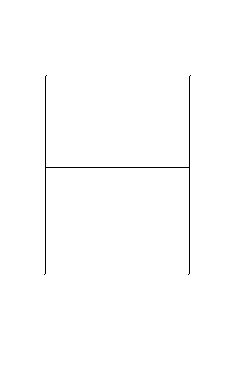
\includegraphics[width=.2\linewidth]{../paper/images/h-skel-inv}};
				\node[draw](k1) at (4,-3.5) {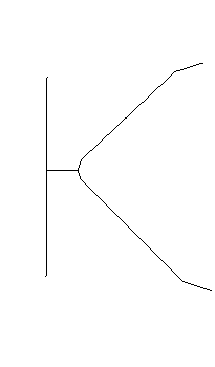
\includegraphics[width=.2\linewidth]{../paper/images/k-skel-inv}};
				\node[draw, label=below:{Skeletons}](z1) at (4,-7) {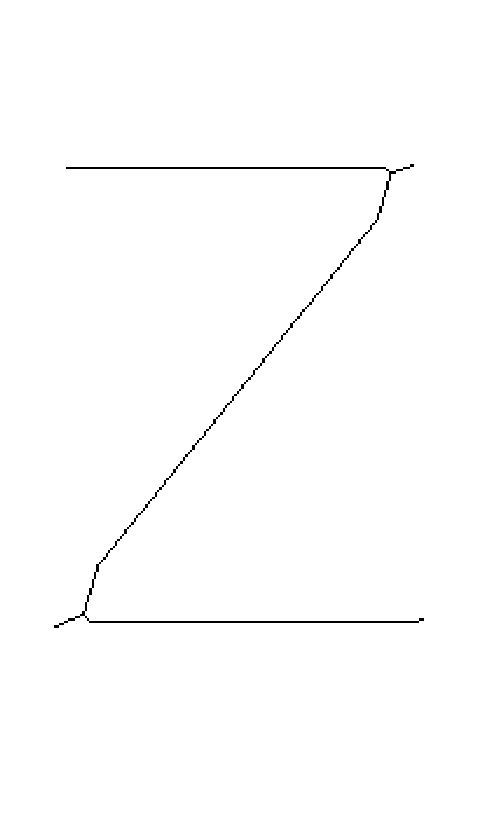
\includegraphics[width=.2\linewidth]{../paper/images/z-skel-inv}};
				
				\node[draw, circle, color=black, fill=bg] (north) at (7,0) {};
				\node[draw, circle, color=black, fill=node] (n0) at (8,-2) {};
				\node[draw, circle, color=black, fill=node] (n1) at (8,-4) {};
				\node[draw, circle, color=black, fill=node] (n2) at (8,-6) {};
				\node[draw, circle, color=black, fill=node] (n3) at (10,-2) {};
				\node[draw, circle, color=black, fill=node] (n4) at (10,-4) {};
				\node[draw, circle, color=black, fill=node] (n5) at (10,-6) {};
				
				\draw[-, ultra thick] (north) to node [midway, fill=bg] {4} (n0);
				\draw[-, ultra thick] (n1) to node [midway, fill=bg] {1} (n0);
				\draw[-, ultra thick] (n1) to node [midway, fill=bg] {1} (n2);
				\draw[-, ultra thick] (n1) to node [midway, fill=bg] {1} (n4);
				\draw[-, ultra thick] (n4) to node [midway, fill=bg] {1} (n3);
				\draw[-, ultra thick] (n4) to node [midway, fill=bg] {1} (n5);
				
				\draw[->, ultra thick] (h0.east) to (h1.west);
				\draw[->, ultra thick] (k0.east) to (k1.west);
				\draw[->, ultra thick] (z0.east) to (z1.west);
				
				\draw[->, ultra thick] (h1.east) to ($(h1.east) + (1.5,-1)$);
				\draw[->, ultra thick] (k1.east) to ($(k1.east) + (1.5,0)$);
				\draw[->, ultra thick] (z1.east) to ($(z1.east) + (1.5,1)$);
				
				\node at (9,-7) {Output Graph};
				\end{tikzpicture}
			}
			
			\vspace{0.5em}
			
			\caption{Characters with isomorphic structure, which are thus ``identical'' \texttt{GlyphGraph} models.\label{fig:badisomorphism}}
		\end{figure}
	\end{column}
	\begin{column}{0.4\linewidth}
		\vspace{0.5em}
		
		We have an issue... these characters are very different to us, yet skeletonisation artifacts add ``tails'' where there should be none.
		
		\pause
		
		\begin{alertblock}{How can we fix this?}
			\begin{enumerate}[<alert@+(1)>]
				\item Convert feature edges into vertices.
				\item Add an edge between feature vertices if they met at the same vertex beforehand.
				\item Label edges with relative path angles!
			\end{enumerate}
		\end{alertblock}
	\end{column}
\end{columns}
\end{frame}

\begin{frame}{A ``Dual'' Representation}
	\begin{figure}
		\definecolor{pixel 0}{HTML}{FFFFFF}
		\definecolor{pixel 1}{HTML}{000000}
		\definecolor{pixel 4}{RGB}{150,227,240}
		\colorlet{pixel 3}{uofglavendar}
		\colorlet{pixel 2}{uofgpumpkin}
		\centering
		\large
		
		\resizebox{\linewidth}{!}{
		\begin{tikzpicture}
		
		\node (old) at (0,0) {
			\resizebox{0.2\linewidth}{!}{
				\begin{tikzpicture}[scale=0.5]		
				\node[draw, circle, color=black, fill=bg] (north) at (3,-1) {};
				\node[draw, circle, color=black, fill=pixel 2] (n0) at (5.5,-1.5) {};
				\node[draw, circle, color=black, fill=pixel 2] (n1) at (6.5,-9.5) {};
				
				\node[draw, circle, color=black, fill=pixel 3] (n2) at (4.5,-5.5) {};
				\node[draw, circle, color=black, fill=pixel 3] (n3) at (7.5,-5.5) {};
				
				\draw[-, ultra thick] (north) to node [midway, fill=bg] {4} (n0);
				
				\draw[-, ultra thick] (n0) to [bend right=90] node [midway, fill=bg] {2} (n1);
				\draw[-, ultra thick] (n0) to [bend left=90] node [midway, fill=bg] {2} (n1);
				
				\draw[-, ultra thick] (n2) to node [midway, fill=bg] {1} (n3);
				
				
				\draw[-, ultra thick] (n0) to node [midway, fill=bg] {3} (n2);
				\draw[-, ultra thick] (n3) to node [midway, fill=bg] {3} (n1);
				\end{tikzpicture}
			}
		};
	
		\node (new) at (4,0) {
			\resizebox{0.3\linewidth}{!}{\begin{tikzpicture}
			\begin{scope}[auto, every node/.style={draw,circle,minimum size=2em,inner sep=1},node distance=2cm]
			\node (n0) at (0,0) {4};
			\node[fill=uofgpumpkin] (n1) at (1.4,1.4) {2};
			\node[fill=uofgpumpkin] (n2) at (1.4,-1.4) {2};
			\node (n3) at (2.8,0) {3};
			
			\node[fill=uofglavendar, text=bg] (n4) at (4.8,0) {1};
			\node (n5) at (6.8,0) {3};
			\end{scope}
			
			\draw[-, ultra thick] (n0) to node [midway, fill=bg] {8} (n1);
			\draw[-, ultra thick] (n0) to node [midway, fill=bg] {8} (n2);
			\draw[-, ultra thick] (n0) to node [near end, fill=bg] {0} (n3);
			
			\draw[-, ultra thick] (n1) to node [near end, fill=bg] {3,4} (n2);
			\draw[-, ultra thick] (n1) to node [midway, fill=bg] {8} (n3);
			
			\draw[-, ultra thick] (n2) to node [midway, fill=bg] {8} (n3);
			
			\draw[-, ultra thick] (n3) to node [midway, fill=bg] {8} (n4);
			
			\draw[-, ultra thick] (n4) to node [midway, fill=bg] {8} (n5);
		
			\draw[-, ultra thick] (n2) to [bend right=30] node [midway, fill=bg] {8} (n5);
			\draw[-, ultra thick] (n1) to [bend left=30] node [midway, fill=bg] {8} (n5);
			\end{tikzpicture}}
		};
	
		\node (txt) at ($(old.east)!0.5!(new.west)$) {\huge $\Rightarrow$};
		
		\end{tikzpicture}
		}
	\end{figure}
	\centering
	Note: relative path dynamics need to be computed during the first transform!
\end{frame}

\section{How Do These Models Perform?}

\begin{frame}{Quickly: Modifications to \alert{$k\downarrow$}}
	These graphs are \alert{attributed multigraphs}: vertices are labelled, and between any vertex pairs we now have a sorted sequence of edge labels.
	I apply top-of-search filtering on vertex labels and loops, and augment propagation to ensure edges are mapped as follows:

	\begin{description}[<alert@+>]
		\item[Non-Induced] Non-induced problem, compatible sequences must share at least one label
		\item[ECI] Edge-count-increasing. Non-induced problem, compatible sequences if there's an injective mapping from pattern sequence to target sequence
		\item[Induced] Induced problem, compatible sequences if equal
	\end{description}	
	
\end{frame}

\begin{frame}{Experiments}
	\begin{enumerate}[<alert@+>]
		\item How do these models handle distinct styles with no variation?
		We can plot dissimilarity dependent on style (Serif vs Sans, Sans vs Sans).
		Is the dual model more distinct?
		Success if GED is around median graph order.
		
		\item Do these models work for large databases of handwritten characters with high variation, the HWRT database?
		Can varying pen radius, line/curve sensitivity enhance accuracy?
		Success if ${}\sim\SI{90}{\percent}$ accuracy.
		
		\item What about small databases of handwritten words with little variation, the George Washington database?
		Are the graphs too big, how do they measure up against state-of-the-art?
		Success if ${}\sim\SI{80}{\percent}$ accuracy---\citeauthor{Graphs-Handwriting}'s result \cite{Graphs-Handwriting}.
	\end{enumerate}
\end{frame}

\begin{frame}{Font Analysis: MCS Variant Choice for DejaVu Sans}
	\begin{figure}
		\centering
		\begin{subfigure}[b]{0.3\linewidth}
			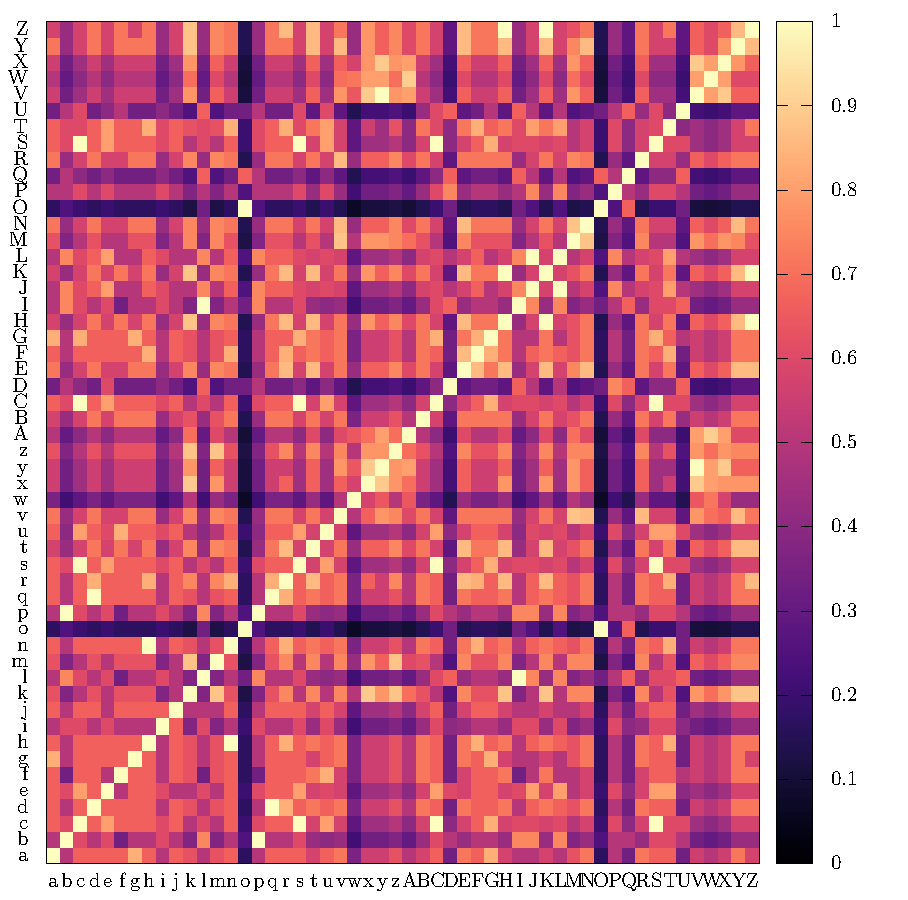
\includegraphics[width=\linewidth, height=0.9\linewidth]{../tables/dejavu-sans/induced-conf-nrm.pdf}
			\caption{
				Induced
				\label{fig:heat:filter:induced}
				%			goop monster quest?
			}
		\end{subfigure}
		\begin{subfigure}[b]{0.3\linewidth}
			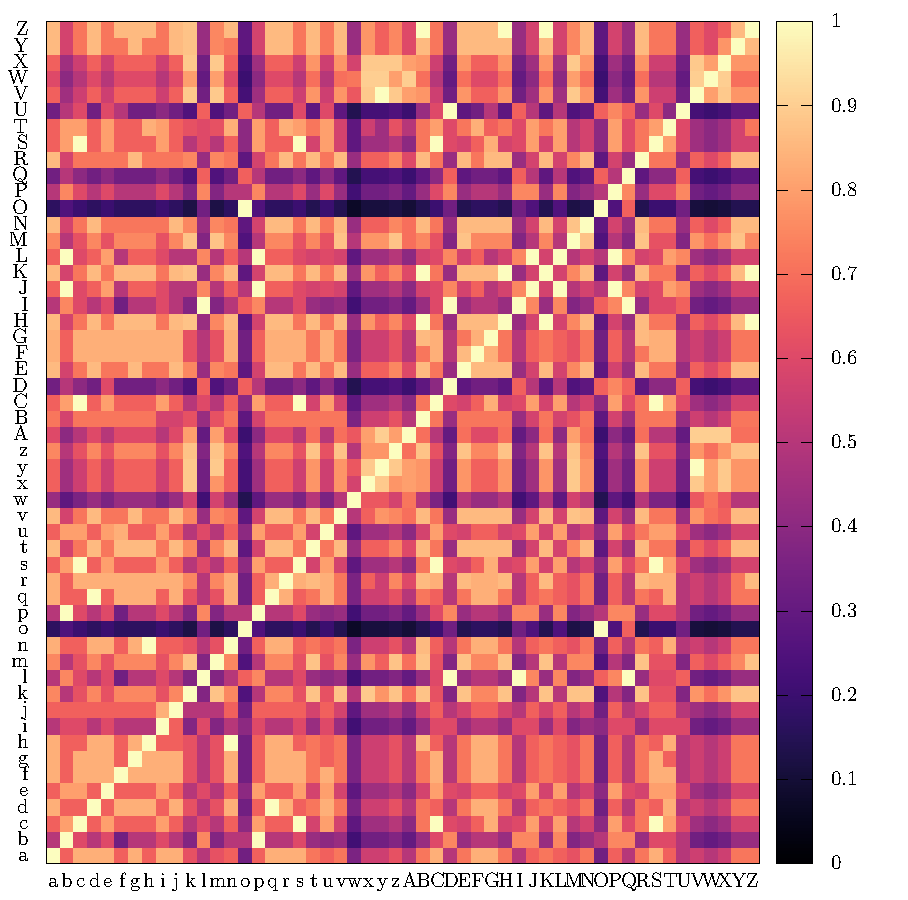
\includegraphics[width=\linewidth, height=0.9\linewidth]{../tables/dejavu-sans/edgecountinc-conf-nrm.pdf}
			\caption{
				ECI
				\label{fig:heat:filter:eci}
				%			smile!
			}
		\end{subfigure}
		\begin{subfigure}[b]{0.3\linewidth}
			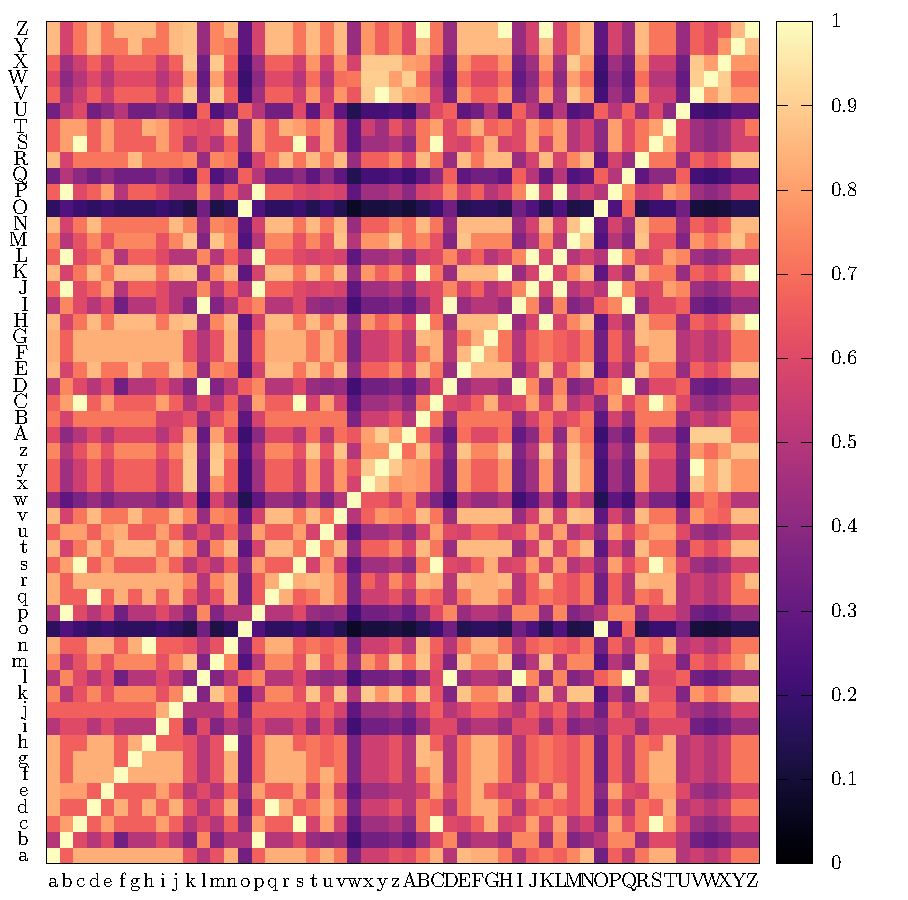
\includegraphics[width=\linewidth, height=0.9\linewidth]{../tables/dejavu-sans/edgecountdec-conf-nrm.pdf}
			\caption{
				%			yes!
				Non-induced
				\label{fig:heat:filter:non-ind}
			}
		\end{subfigure}
	\end{figure}

	Heatmaps showing $\text{Ord}(\textit{MCS})$, normalised.
	These show the same trends as GED, which does hover around median size for all but serif fonts, but far clearer.
	Brightness implies similarity, which we only want on the diagonal if possible!
	
	The \alert{induced variant is best on this problem}: it has the fewest unintended isomorphisms, and higher dissimilarity across the board.
\end{frame}

\begin{frame}{Font Analysis: Regular vs Dual for DejaVu Sans (Induced)}
	\begin{figure}
		\centering
		\begin{subfigure}[b]{0.4\linewidth}
			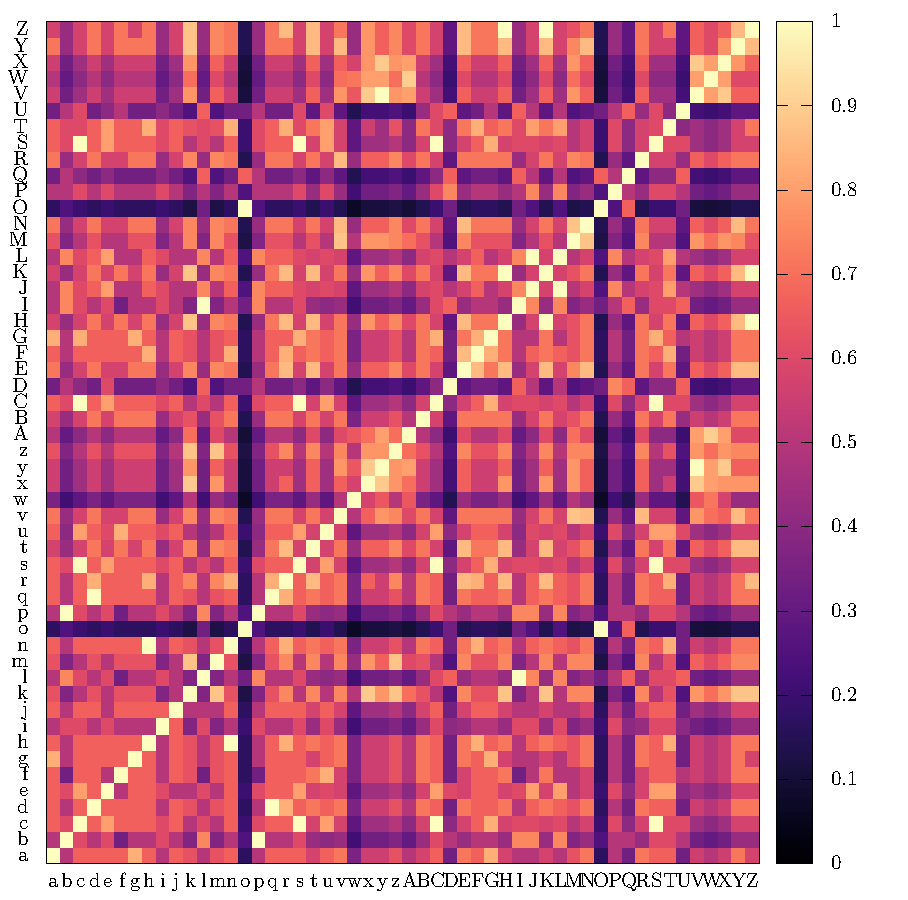
\includegraphics[width=\linewidth, height=0.9\linewidth]{../tables/dejavu-sans/induced-conf-nrm.pdf}
			\caption{
				Regular
			}
		\end{subfigure}
		\begin{subfigure}[b]{0.4\linewidth}
			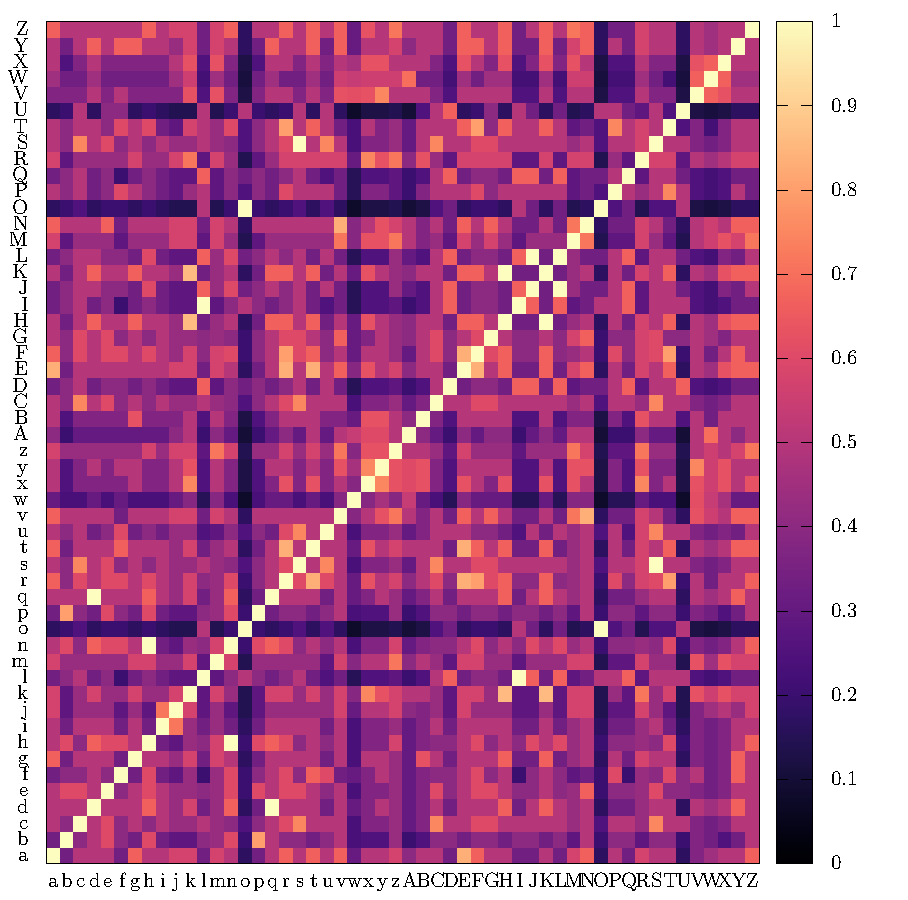
\includegraphics[width=\linewidth, height=0.9\linewidth]{../tables/dual-dejavu-sans/induced-conf-nrm.pdf}
			\caption{
				Dual
			}
		\end{subfigure}
	\end{figure}
	
	Same criteria---within this font, we see that the ``Dual'' representation removes further isomorphisms (but not all, implying a need for scale-encoding features).
	For now, the ``Dual'' representation is successful; \alert{the graph models allowed us to intuit what was wrong, and correct for it.}
\end{frame}

\begin{frame}{Font Analysis: Open Sans vs DejaVu Sans (Induced)}
	\begin{figure}
		\centering
		\begin{subfigure}[b]{0.4\linewidth}
			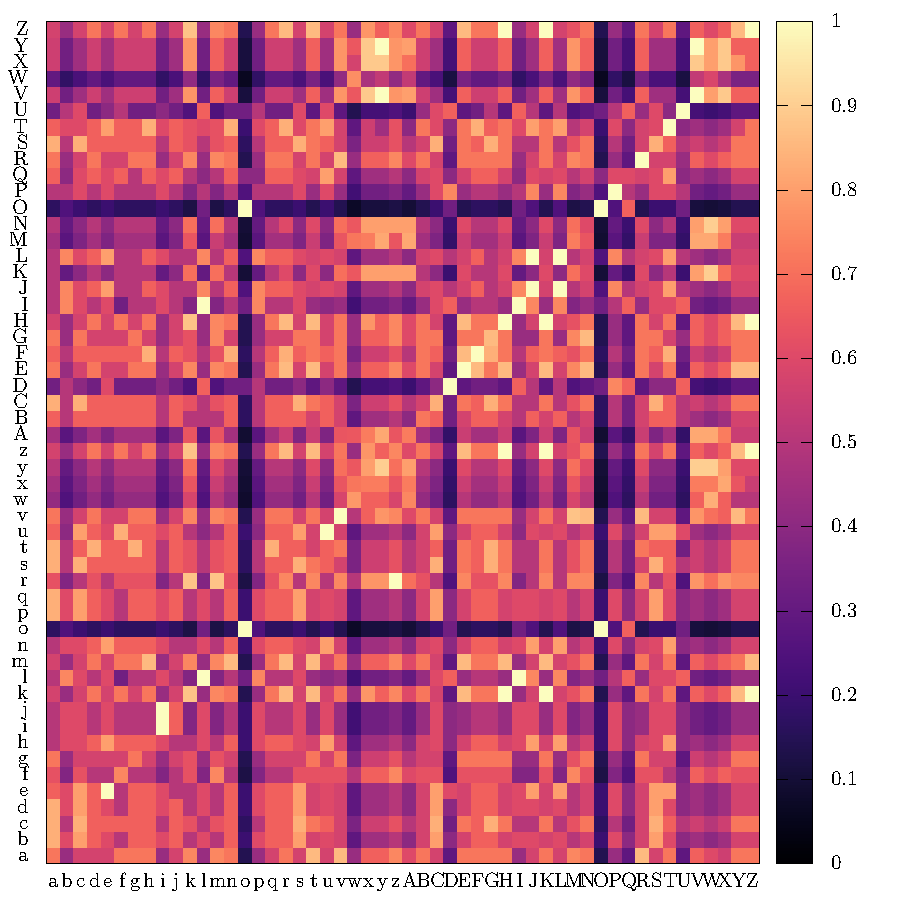
\includegraphics[width=\linewidth, height=0.9\linewidth]{../tables/open-sans-dejavu-sans/induced-conf-nrm.pdf}
			\caption{
				Regular
			}
		\end{subfigure}
		\begin{subfigure}[b]{0.4\linewidth}
			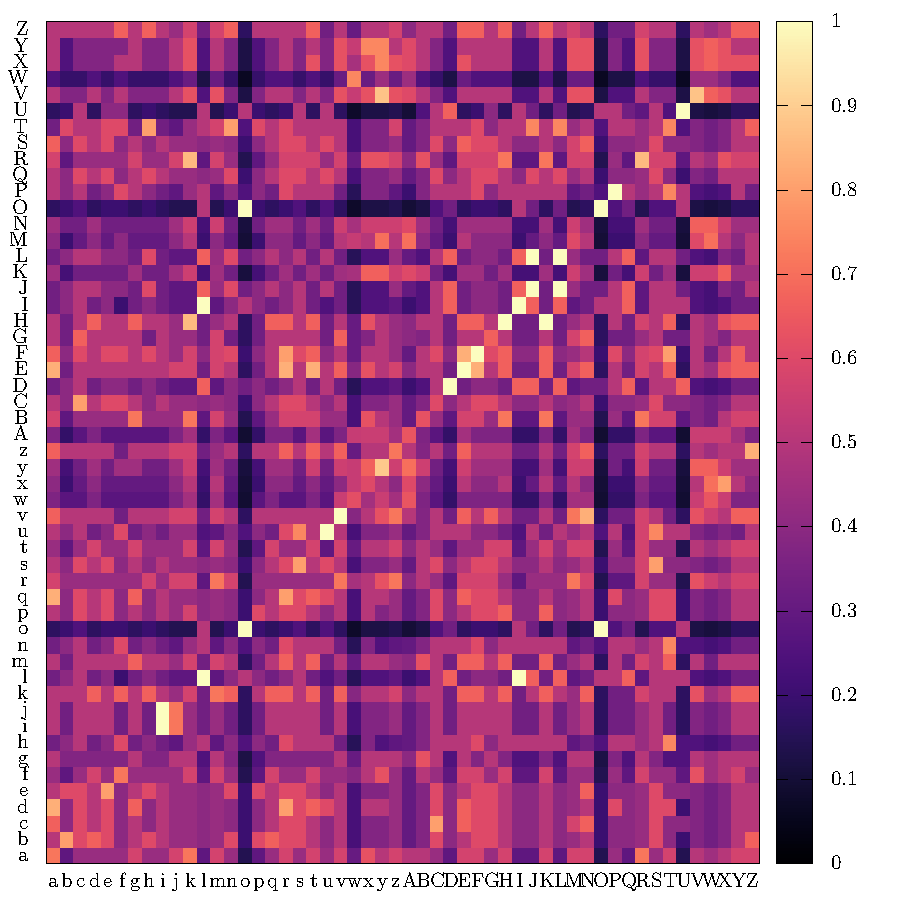
\includegraphics[width=\linewidth, height=0.9\linewidth]{../tables/dual-open-sans-dejavu-sans/induced-conf-nrm.pdf}
			\caption{
				Dual
			}
		\end{subfigure}
	\end{figure}

	Some isomorphisms are preserved between fonts, but relatively few.
	Examining the graphs shows different path splitting behaviour due to minor curvature variations---this does not bode well for \emph{matching between styles} of glyphs.
	
\end{frame}

\begin{frame}{Font Analysis: Open Sans vs Alegreya (Induced)}
	\begin{figure}
		\centering
		\begin{subfigure}[b]{0.4\linewidth}
			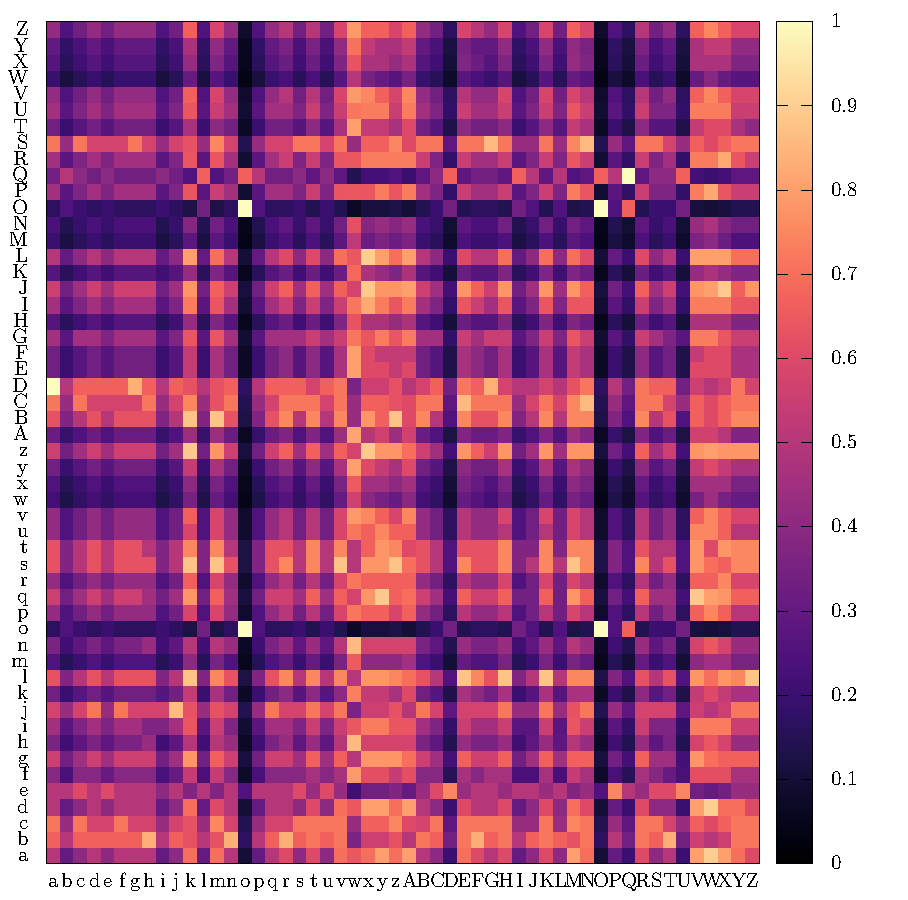
\includegraphics[width=\linewidth, height=0.9\linewidth]{../tables/alegreya-dejavu-sans/induced-conf-nrm.pdf}
			\caption{
				Regular
			}
		\end{subfigure}
		\begin{subfigure}[b]{0.4\linewidth}
			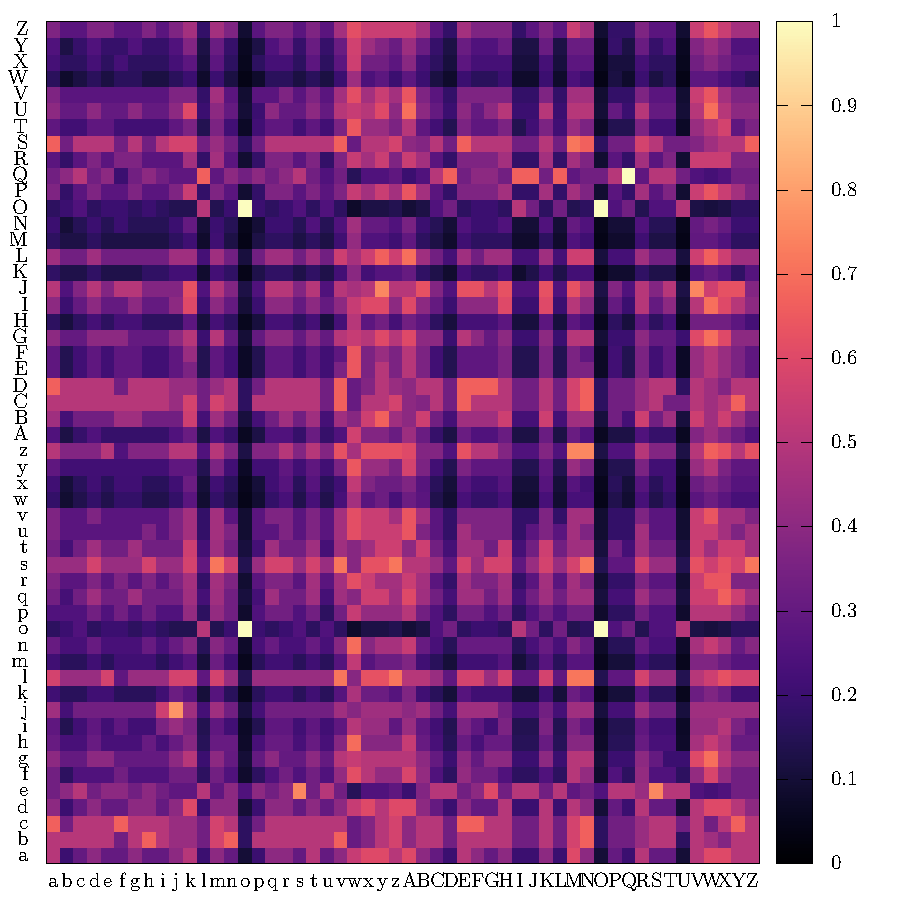
\includegraphics[width=\linewidth, height=0.9\linewidth]{../tables/dual-alegreya-dejavu-sans/induced-conf-nrm.pdf}
			\caption{
				Dual
			}
		\end{subfigure}
	\end{figure}
	
	Virtually no isomorphisms, or matching power.
	Serifs on letters greatly inflate graph order and completely change neighbourhood and orientation dynamics.
\end{frame}

\begin{frame}[standout]
	It's \alert{easy to achieve better performance for distinct tasks}, and we can see what might aid matching due to the intuitive models.
	
	However, we see \alert{poor performance matching between character styles}.
	Is this indicative of classifier performance?
\end{frame}

\begin{frame}{Handwritten Data: $k$NN on HWRT}
\begin{columns}
	\begin{column}{0.3\textwidth}
		\vspace{-2em}
		\begin{table}
			\centering
			\resizebox{\linewidth}{!}{
			\begin{tabular}{SSS}
				\toprule
				\multicolumn{1}{c}{$r$ (px)} & \multicolumn{1}{c}{Accuracy (\si{\percent})} & \multicolumn{1}{c}{$\kappa$} \\
				\midrule
				1 & 38.46 & 0.347 \\
				5 & 29.86 & 0.256 \\
				9 & 30.77 & 0.271 \\
				\bottomrule
			\end{tabular}
			}
			\vspace{-0.5em}
			\caption{
%				\scriptsize
				Regular Model, Induced
			}
		\end{table}
		
		\vspace{-2.5em}
		\begin{table}
			\centering
			\resizebox{\linewidth}{!}{
			\begin{tabular}{SSS}
				\toprule
				\multicolumn{1}{c}{$r$ (px)} & \multicolumn{1}{c}{Accuracy (\si{\percent})} & \multicolumn{1}{c}{$\kappa$} \\
				\midrule
				1 & 34.84 & 0.312 \\
				5 & 27.15 & 0.233 \\
				9 & 26.24 & 0.222 \\
				\bottomrule
			\end{tabular}
			}
			\vspace{-0.5em}
			\caption{
%				\scriptsize
				Dual Model, Induced
			}
		\end{table}
		
		\vspace{-2.5em}
		\begin{table}
			\centering
			\resizebox{\linewidth}{!}{
			\begin{tabular}{SSS}
				\toprule
				\multicolumn{1}{c}{$\mathit{curve\_thr}$} & \multicolumn{1}{c}{Accuracy (\si{\percent})} & \multicolumn{1}{c}{$\kappa$} \\
				\midrule
				1.2 & 40.72 & 0.373 \\
				1.35 & 38.46 & 0.347 \\
				1.5 & 38.46 & 0.347 \\
				1.65 & 35.75 & 0.318 \\
				\bottomrule
			\end{tabular}
			}
			\vspace{-0.5em}
			\caption{
%				\scriptsize
				Curve Sensitivity (Regular, Induced, $r=1$)
			}
		\end{table}
	\end{column}
	\begin{column}{0.7\textwidth}
		\vspace{-3em}
		\begin{itemize}
			\item \emph{$k$-Nearest Neighbours} classifier, using GED
			\item Median $\text{Ord}(\mathcal{G})$ is 6--7, $\text{Sz}(\mathcal{G})$ is 6--8
			\item Lower pen-radius better, less connections in places but more representative
			\item Induced better (again), but 6--8 times longer runtime
			\item Regular better than dual, since it captures a very rigid notion of path dynamics
			\item Higher curve sensitivity is better, due to earlier weaknesses
			\item \alert{Peak performance of \SI{40.72}{\percent}}
			\item Hasn't been before tested with graph models, so no reference point
		\end{itemize}
	\end{column}
\end{columns}
\end{frame}

\begin{frame}{Handwritten Data: $k$NN on George Washington}
	\begin{itemize}
		\item Regular median $\text{Ord}(\mathcal{G})$ is 33, $\text{Sz}(\mathcal{G})$ is 42
		\item For Dual, median $\text{Ord}(\mathcal{G})$ is 42, $\text{Sz}(\mathcal{G})$ is 75
		\item Long story short, these graphs are \alert{far too large to operate on} as they model whole words!
		\item \citeauthor{Graphs-Handwriting} use approximate distance metrics, I'd hoped that these models would be more compact than existing approaches based on adaptive segmentation
		\item \alert{Peak performance... \SI{11.67}{\percent} (ouch!)}
		\item ...did this issue jeopardise the prior experiment?
	\end{itemize}
\end{frame}

\begin{frame}[standout]
	There is \emph{some} value in these models, but the somewhat intuitive additions are a double-edged sword.
	The dual model \alert{overfits} to font data, so it is a poor (and costly) fit for handwriting! 

	Exact graph comparisons are too expensive in practice, this is a source of uncertainty in these results.
\end{frame}

\section{Conclusions}

%\begin{frame}[standout]
%Conclusion!
%\end{frame}

\begin{frame}{Conclusion}
	\begin{itemize}[<+- | alert@+>]
		\item Existing general image graph models are not appropriate or effective!
		\item The demonstrated models are generally pretty poor but...
		\item They are easily modifiable, and we can always have a good sense of what the machine is seeing and why!
		\begin{itemize}
			\item This makes it easier to \emph{overfit} to any dataset, however...
		\end{itemize}
		\item Future work? Apply others' techniques to HWRT dataset, examine approximate GED with my own, and consider custom cost metrics to make certain features ``more important''
	\end{itemize}
	
	\pause
	
	\only<6->{\alert{\textbf{Any questions?}}}
\end{frame}

\appendix

\begin{frame}[allowframebreaks]{References}

\printbibliography[heading=none]

\end{frame}

\end{document}